\chapter{Introduction}


\section{Star-galaxy Classification in Photometric Surveys}


Currently ongoing and upcoming large-scale surveys, such as the Dark Energy Survey (DES)
and the Large Synoptic Survey Telescope (LSST), are purely photometric surveys,
where digital images of the sky are obtained and subsequently analyzed.
To quantify the brightness of a source in a photometric image,
we count the number of photons from the source within a fixed aperture
(\eg a circle or a two-dimensional Gaussian).
This brightness measurement is expressed in units of magnitude ---
a logarithmic unit in which the fainter a source appears the larger its magnitude.
In mathematical terms, the apparent magnitude $m$ in a spectral band $\lambda$ is given by
\begin{equation}
m_{\lambda} = - 2.5 \log_{10} \frac{ F_{\lambda} }{ F_{\lambda,0} },
\end{equation}
where $F_{\lambda}$ is the observed flux using the photometric filter $\lambda$ ,
and $F_{\lambda,0}$ is the reference flux (\ie zero-point) for that filter.
Photometric surveys use filters on telescopes to allow only light around
a specific wavelength to pass.
Figure~\ref{fig:filters} shows the wavelengths of the five filters (named $u$, $g$, $r$, $i$, $z$)
of the Sloan Digital Sky Survey (SDSS).
Before these photometric data can be used for a scientific analysis, however, they must be classified,
which for most sources is either a star or a galaxy.

Stars are in our Milky Way galaxy and are close to us compared to distant galaxies.
Due to their small physical size, however, almost all stars appear as compact point sources
in photometric images.
Galaxies, despite being farther away, generally subtend a larger angle, and thus
appear as extended sources.
However, as Figure~\ref{fig:sg_mag} demonstrates, it becomes increasingly difficult
to separate stars from galaxies due to a large number of unresolved galaxies at faint magnitudes.
Since the number of galaxies grows exponentially with magnitude, 
this implies that the majority of sources that are detected in the current and
next-generation ground-based surveys may be challenged by poor star-galaxy classification.
Furthermore, due to the sheer number of stars and galaxies,
this classification has to be automated.
For example, the SDSS has obtained photometric observations of more than $3 \times 10^8$ objects
\citep{eisenstein2011sdss},
and the LSST will produce a catalog of $2 \times 10^{10}$ galaxies and a similar number of stars
\citep{ivezic2008lsst}.
Thus, there is a need for a robust, automated classification technique for large ground-based photometric surveys.

The classification of stars vs.\ galaxies has many important applications in precision cosmology.
As a basic example, in a homogeneous universe with a Euclidean geometry for three-dimensional space,
the number counts of galaxies as a function of magnitude follows
\begin{equation}
N \left( m_{\lambda} \right) \propto 10^{ 0.6 \left( m_{\lambda} - m_{\lambda,0} \right) }.
\end{equation}
By comparing this relation with the predictions of a Friedmann-Robertson-Walker (FRW) universe
(\ie the standard model of cosmology),
\citet{yasuda2001galaxy} show that our universe does not have a Euclidean geometry for
three-dimensional space.
Without a reliable method for separating stars from unresolved galaxies, 
we risk underestimating the number density of galaxies by rejecting all unresolved galaxies,
while including them could result in significant contamination of the galaxy sample.
Furthermore, the accurate separation of stars and galaxies in faint samples
significantly improves our ability to
(i) measure auto-correlation functions of luminous galaxies \citep{ross2011ameliorating},
(ii) control the systematic errors in the weak lensing shear measurement \citep{soumagnac2015star},
(iii) map the signature of baryon acoustic oscillations \citep{anderson2014clustering}, and
(iv) identify electromagnetic counterparts to gravitational wave sources \citep{miller2017preparing},
among other things.

Given the importance of this classification problem, it is not surprising that a variety of
different strategies have been developed.
The most commonly used method to classify stars and galaxies in large sky surveys is the morphological separation
\citep{sebok1979optimal, kron1980photometry, valdes1982resolution, yee1991faint, vasconcellos2011decision,
henrion2011bayesian}.
It relies on the assumption that stars appear as point sources while galaxies appear as resolved sources.
For example, a popular technique in the weak lensing community \citep{Kaiser1995}
makes a hard cut in the space of photometric attributes as shown in Figure \ref{fig:intro_morc}.
As the Figure shows, there is a distinct locus
produced by point sources in the half-light radius vs.\ the $i$-band magnitude plane.
(The half-light radius is the effective radius at which half of the total light of an object is contained.)
A rectangular cut in this size-magnitude plane separates point sources
(which are presumed to be stars) from resolved sources (which are presumed to be galaxies).

However, such a hard cut in a low-dimensional parameter space has disadvantages:
it does not break down gracefully; its treatment of measurement uncertainties is too simplistic;
it uses a rather limited subset of the full information available;
and it ignores a priori information like the expected demographics of the source populations.
Furthermore, currently ongoing and upcoming large photometric surveys
will detect a vast number of unresolved galaxies at faint magnitudes.
Near a survey's limit, the photometric observations cannot reliably separate stars from unresolved galaxies
by morphology alone without leading to incompleteness and contamination in the star and galaxy samples.

\section{Machine Learning}

\subsection{Supervised Learning}

The systematic misclassification of sources can be mitigated by using machine learning algorithms.
Machine learning methods have the advantage that it is easier to include extra information,
such as shape information or different model magnitudes.
Machine learning techniques are usually categorized into two main types: supervised and unsupervised learning approaches.
In the supervised learning approach, the input attributes (\ie the values that describe the properties of each objects \eg magnitudes),
$\mathbf{X}= \{ \mathbf{x}_1,\mathbf{x}_2,\dots,\mathbf{x}_N \}$,
are provided along with the desired output values (\eg star or galaxy),
$\mathbf{y} = \{ y_1, y_2, \dots, y_N \}$, in a labeled set of input-output pairs
$\mathbf{D} = \{ \left( \mathbf{x}_i, y_i \right) \}_{i = 1}^N$.
Here, $\mathbf{D}$ is the training set, and $N$ is the number of training examples.
The goal of supervised learning is then to estimate a function that maps $f: \mathbf{X} \rightarrow \mathbf{y}$.
As we discuss in the following chapters, it is desirable for the algorithm to return a probability.
To emphasize the need for probabilistic predictions, we formulate the goal of supervised learning as folows:
a probabilistic supervised learning algorithm infers the probability distribution $P( \mathbf{y} | \mathbf{X}, \mathbf{D} )$
over possible labels, given the input $\mathbf{X}$ and training set $\mathbf{D}$.
We use the conditioning bar $|$ to explicitly show that the probability is conditional on both
the input $\mathbf{X}$ and the training set $\mathbf{D}$.
When we have a set of multiple models to choose from, we explicitly condition the probability on the set of models and write
$P \left( \mathbf{y} | \mathbf{X}, \mathbf{D}, \mathbf{M} \right)$, where $\mathbf{M}$ is the set of models.
However, if it is clear from the context which model we use to make predictions, we drop $\mathbf{M}$ although
it is implied that the probability is conditional on the form of model.

To obtain the truth labels for the training data,
we use spectroscopy to measure the spectrum of electromagnetic radiation
from stars and galaxies.
Although modern spectrometers are more complex,
a spectrometer, in its most basic form, consists of a slit,
a prism or diffraction grating (to split the light into its component colors), and a detector.
We can use spectroscopy to measure many properties of distant stars and galaxies,
such as their chemical composition, temperature, and distance, and thus
spectral classification can be used as the ground truth for classifying sources in photometric images.

\subsection{Neural Networks}

As an example of a supervised learning algorithm, we provide a brief description of
\textit{artificial neural networks} (ANN)---the most widely used machine learning algorithm in astronomy.
The use of neural networks in astronomy goes as far back as the mid 1980s \citep{jeffrey1986optimization}.
ANN was first applied to the star-galaxy classification problem by \citet{odewahn1992automated},
and it has become a core part of the popular astronomical image processing software \textsc{SExtractor}~\citep{bertin1996sextractor}.

The original motivation for ANNs was to simulate neurons in the human brain.
A neuron in the human brain receives signals from other neurons through synaptic connections.
If the combination of these signals exceeds a certain threshold,
the neuron will fire and send a signal to other neurons.
Intelligence is believed to be the collective effect of
approximately $10^{11}$ neurons firing.
An artificial neuron in most artificial neural networks is represented
as a mathematical function that models a biological neural structure
(Figure~\ref{fig:intro_neuron_a}).
Let $\mathbf{x}=\left(x_1,x_2,\dots,x_n\right)$ be a vector of inputs to a given neuron,
$\mathbf{w}=\left(w_1,w_2,\dots,w_n\right)$ be a vector of weights, and
$b$ be the bias.
Then, the output of the neuron is
\begin{equation}
  y = \sigma \left( \mathbf{w} \cdot \mathbf{x} + b \right),
  \label{eq:intro_neuron_output}
\end{equation}
where $\sigma$ is the activation function (or \textit{non-linearity}).
Common activation functions include the sigmoid function,
\begin{equation}
\sigma(x)=1/\left(1+e^{-x}\right),
\end{equation}
the hyperbolic tangent function,
\begin{equation}
\sigma(x)=\tanh(x),
\end{equation}
and the rectified linear unit \citep[ReLU;][]{nair2010rectified},
\begin{equation}
\sigma(x)=\max(0, x).
\end{equation}
Typical neurons are organized as layers, where each neuron in one layer is connected to the neurons of the subsequent layer.
A schematic representation is shown in Figure~\ref{fig:intro_neuron_b}.
All layers except the input and output layers are conveniently called hidden layers.

The training uses an algorithm to a set of weights and biases such that, given $N$ samples, the output from the network
$\mathbf{y}=\left(\hat{y}_1, \hat{y}_2, \dots, \hat{y}_N \right)$
approximates the desired output
$\mathbf{y} = \left(y_1, y_2, \dots, y_N \right)$
as closely as possible for all input
$\mathbf{X}=\left(\mathbf{x}_1,\mathbf{x}_2,\dots,\mathbf{x}_N\right)$.
We can formulate this as the minimization of a loss function $L(\mathbf{y},\hat{\mathbf{y}})$ over the training data.
A common form of the loss function is the \textit{cross-entropy},
\begin{equation}
  L(y_j, \hat{y}_j) = - \frac{1}{N} \sum_{j=1}^{N} y_j  \log_2 \hat{y}_j
    + (1 - y_j)  \log_2 (1 - \hat{y}_j).
  \label{eq:intro_cross_entropy}
\end{equation}
where $y_j$ is the actual truth value (\eg 0 or 1) of the $j$-th data, and
$\hat{y}_j$ is the probability prediction made by the model.

To find the weights $\mathbf{w}$ and biases $\mathbf{b}$ which minimize the loss,
we use a technique called \textit{gradient descent},
where we use the following rules to update the parameters in each layer $l$:
\begin{align}
  \mathbf{w}_l &\rightarrow
  \mathbf{w}_l^{\prime}
  = \mathbf{w}_l - \eta \frac{\partial L}{\partial \mathbf{w}_l} \nonumber \\
  \mathbf{b}_l &\rightarrow
  \mathbf{b}_l^{\prime}
  = \mathbf{b}_l - \eta \frac{\partial L}{\partial \mathbf{b}_l},
  \label{eq:intro_gradient_descent}
\end{align}
where $\eta$ is a small, positive number known as the \textit{learning rate}.
The gradients in \ref{eq:intro_gradient_descent} can be computed using the
\textit{backpropagation} procedure~\citep{rumelhart1988learning},
which is nothing more than an application of the chain rule for derivatives.

\subsection{Unsupervised and Semi-supervised Learning}

In contrast to supervised learning, in which the truth labels are provided,
unsupervised learning does not utilize the desired output during the learning process.
Instead, we are only given unlabeled inputs $\mathbf{D}= \{ \mathbf{x}_i \}_{i=1}^N$,
and the data is clustered into different classes or categories.
In other words, unsupervised learning attempts to infer the probability distribution of the form $P(\mathbf{x}_i)$.
Unsupervised machine learning techniques are less common, in part due to the successes of purely supervised learning.
Semi-supervised learning falls between supervised learning, where training data are completely labeled,
and unsupervised learning, where all training data are unlabeled.
Semi-supervised techniques make use of a large amount of unlabeled data, in conjunction with a small amount of labeled data,
to better capture the underlying data distribution.
We expect unsupervised and semi-supervised learning to become more important, since
it is unclear if sufficient training data will be available in future ground-based photometric surveys and
there will be many orders of magnitude more unlabeled than labeled data available in future ground-based imaging surveys.

\section{Thesis Structure}

In the following chapters, we explore a variety of statistical and machine learning approaches to push the limits of
star-galaxy classification in ground-based photometric surveys.
Each chapter is self-contained and has its own references.

In Chapter~\ref{chapter2}, we present a novel meta-classification
framework that combines and fully exploits different techniques
to produce a more robust star-galaxy classification.
To demonstrate this hybrid, ensemble approach,
we combine a purely morphological classifier,
a supervised machine learning method based on random forest,
an unsupervised machine learning method based on self-organizing maps,
and a hierarchical Bayesian template fitting method.
Using data from the Canada-France-Hawaii Telescope Lensing Survey (CFHTLenS),
we consider different scenarios:
when a high-quality training set is available with spectroscopic labels,
and when the demographics of sources in a low-quality training set
do not match the demographics of objects in the test data set.
We demonstrate that our Bayesian combination technique improves
the overall performance over any individual classification method
in these scenarios.

In Chapter~\ref{chapter3}, we present a star-galaxy classification framework that uses a supervised machine learning algorithm called
convolutional neural networks (ConvNets).
Most existing star-galaxy classifiers use the reduced summary information from catalogs,
requiring careful feature extraction and selection.
Deep ConvNets allow a machine to automatically learn the features directly from images,
minimizing the need for input from human experts.
Using data from the SDSS and CFHTLenS,
we demonstrate that ConvNets are able to produce accurate and well-calibrated probabilistic classifications that are competitive with
conventional machine learning techniques.

In Chapter~\ref{chapter4}, we study the application of a deep learning technique called generative adversarial networks (GANs)
to the star-galaxy classification problem in a semi-supervised setting.
As current and forthcoming photometric surveys probe large cosmological volumes,
the majority of photometric observations are too faint for a uniform spectroscopic follow-up.
As a result, the number of unlabeled data available for training machine learning algorithms will be orders of magnitude
greater than the number of labeled data.
Semi-supervised learning techniques are of great interest since they are able to capture the underlying data distribution
with only a small amount of labeled data.
Using photometric images from the SDSS, we demonstrate that semi-supervised GANs are able to produce
accurate and well-calibrated classifications using only a small amount of labeled examples.
We also show that the number count distributions of the images generated by GAN follow a similar distribution to
the SDSS photometric sample.

In Chapter \ref{chapter5}, we outline our conclusions.

\newpage
\section{Figures and Tables}

\vspace{100pt}

\begin{figure}[htp]
  \centering
  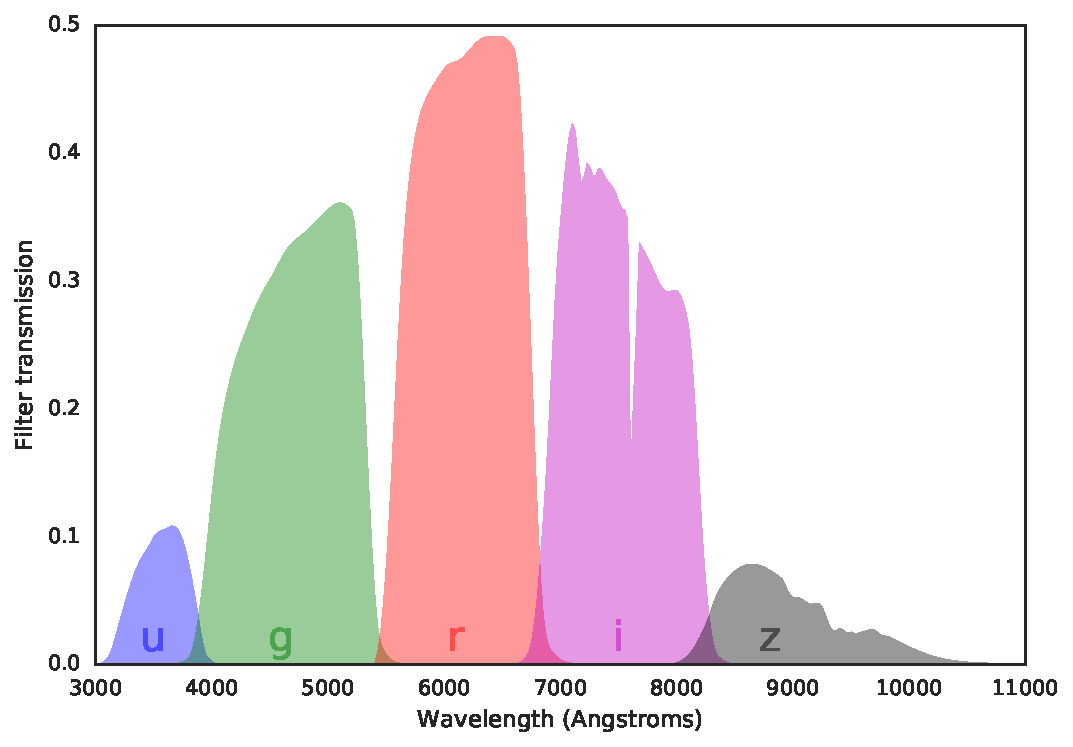
\includegraphics[width=0.8\textwidth]{figures/filters.pdf}
  \caption{The SDSS $ugriz$ filter transmission curves.}
  \label{fig:filters}
\end{figure}

\begin{sidewaysfigure}[htp]
  \centering
  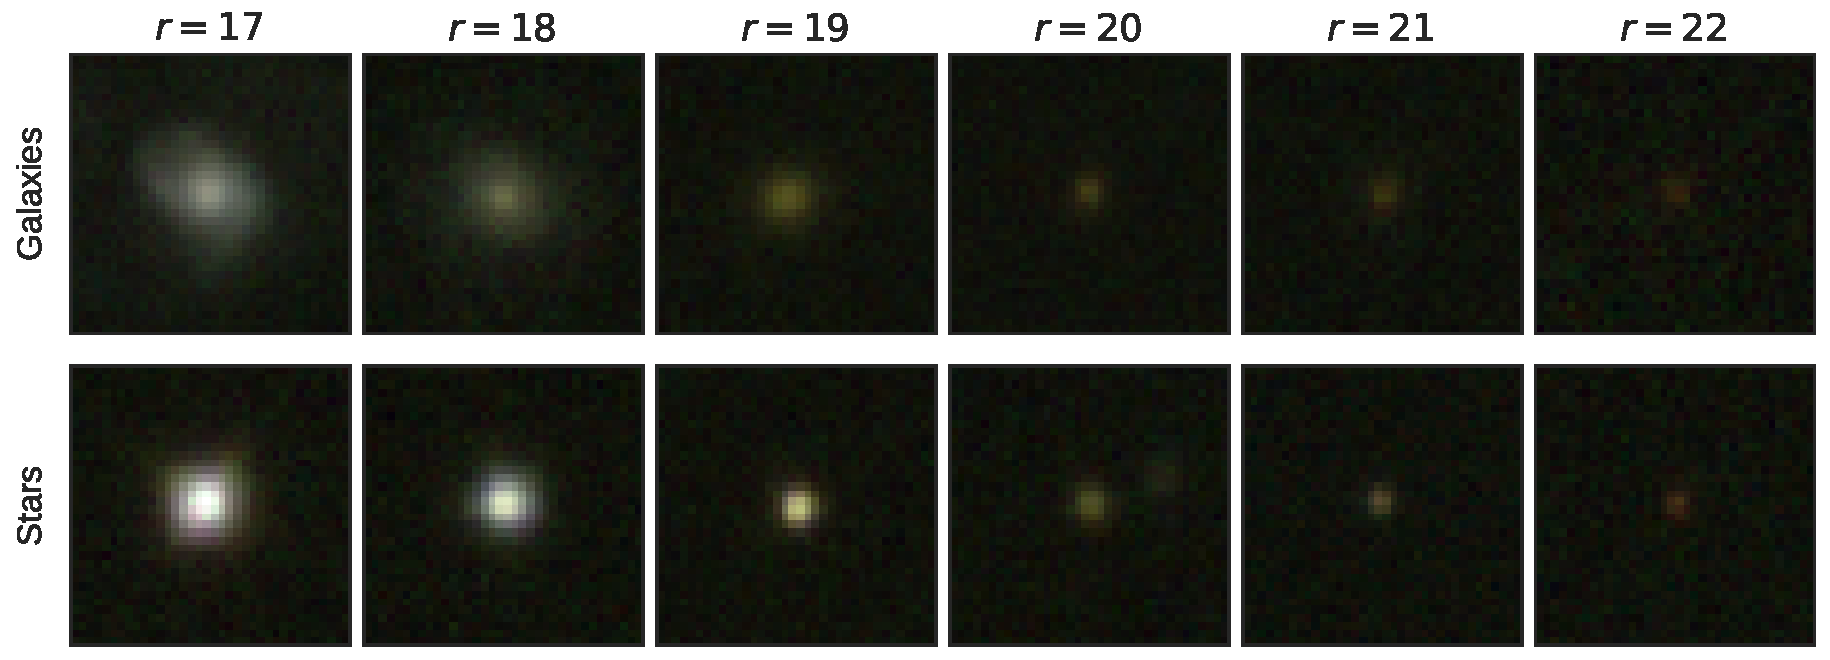
\includegraphics[width=\textwidth]{figures/sgstamps.pdf}
  \caption{Sample images of stars (top row) and galaxies (bottom row) from the SDSS survey
  at different magnitudes ($r$-band).
  Note that it becomes increasingly difficult to classify sources at fainter magnitudes,
  where we have the majority of the detected sources.}
  \label{fig:sg_mag}
\end{sidewaysfigure}

\begin{figure}[htp]
  \centering
  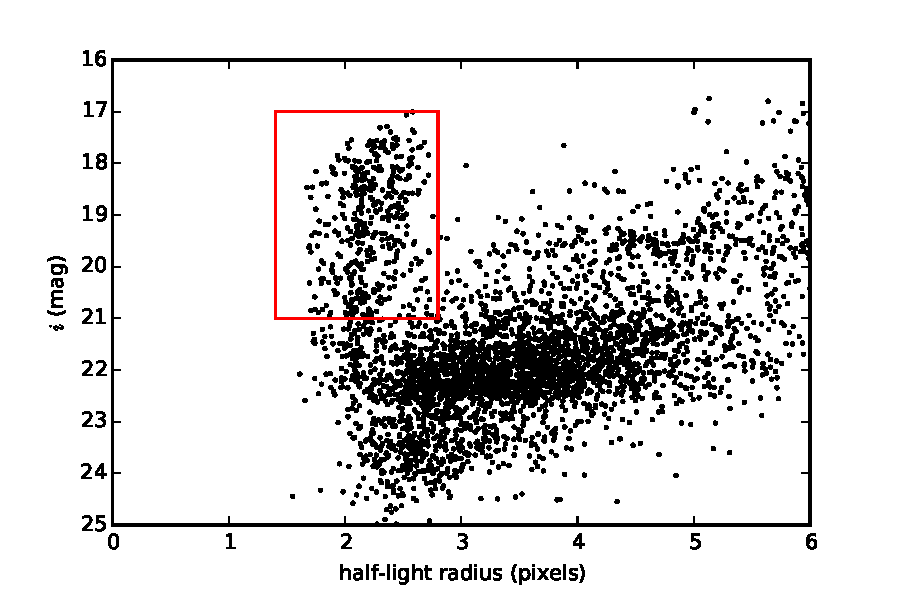
\includegraphics{figures/morph.pdf}
  \caption{Half-light radius vs.\ magnitude.}
  \label{fig:intro_morc}
\end{figure}

\begin{sidewaysfigure}
  \centering
  \begin{subfigure}[]{0.49\linewidth}
    \centering
    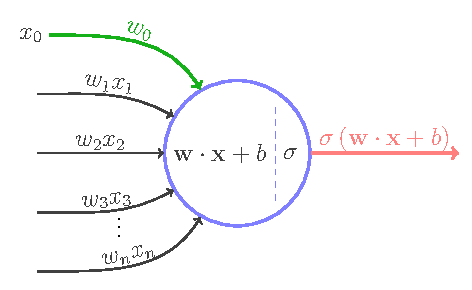
\includegraphics[width=0.6\textwidth]{figures/neuron.pdf}
    \caption{}
    \label{fig:intro_neuron_a}
  \end{subfigure}
  \begin{subfigure}[]{0.49\linewidth}
    \centering
    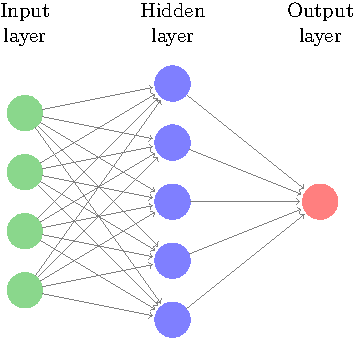
\includegraphics[width=0.6\textwidth]{figures/network.pdf}
    \caption{}
    \label{fig:intro_neuron_b}
  \end{subfigure}
  \caption{
    (a) A mathematical model of a biological neuron.
    (b) A schematic diagram of a neural network with one hidden layer.
    }
\end{sidewaysfigure}


\clearpage
\bibliographystyle{plainnat}
\bibliography{thesisbib}